\section{Unification of Alternative Formulations}\label{sec:alternative_formulations}

The third major open problem, unifying the various formulations of test ideals in mixed characteristic through the binary p-adic framework, is addressed here. Several different formulations of test ideals have been proposed in mixed characteristic, including standard, trace-based, perfectoid, and tight closure formulations. Our goal is to understand precisely when these formulations agree and when they differ.

\subsection{Overview of Alternative Formulations}

We begin by recalling the different formulations of test ideals in mixed characteristic:

\begin{definition}[Standard Test Ideal]\label{def:standard-test-ideal}
The standard test ideal $\tau_{\text{standard}}(R,\Delta)$, introduced by Ma and Schwede \cite{MS18}, is defined using the plus closure as:
$$\tau_{\text{standard}}(R,\Delta) = \bigcap_{f: Y \to \text{Spec}(R)} \text{Tr}_f(f_*\mathcal{O}_Y(K_Y - \lfloor f^*\Delta\rfloor))$$
where the intersection runs over all finite morphisms $f$ from normal integral schemes $Y$ to $\text{Spec}(R)$.
\end{definition}

\begin{definition}[Trace-based Test Ideal]\label{def:trace-test-ideal}
The trace-based test ideal $\tau_{\text{trace}}(R,\Delta)$, studied by McKenzie and Rincon \cite{MR18} and further developed by Quy and Shimomoto \cite{QS17}, modifies the standard definition by imposing additional conditions on the trace map:
$$\tau_{\text{trace}}(R,\Delta) = \bigcap_{f \in \mathcal{F}} \text{Tr}_f(f_*\mathcal{O}_Y(K_Y - \lfloor f^*\Delta\rfloor))$$
where $\mathcal{F}$ is a restricted class of finite morphisms with specific trace properties.
\end{definition}

\begin{definition}[Perfectoid Test Ideal]\label{def:perfectoid-test-ideal-expanded}
The perfectoid test ideal $\tau_{\text{perf}}(R,\Delta)$, developed in the work of André, Bhatt, Morrow, and Tsuji \cite{AMBT19} and refined by Bhatt and Scholze \cite{BS22}, is defined using perfectoid algebras:
$$\tau_{\text{perf}}(R,\Delta) = \{x \in R \mid x \cdot \mathcal{A}(R_{\perfectoid}, \Delta) \subseteq R\}$$
where $\mathcal{A}(R_{\perfectoid}, \Delta)$ is an almost ideal in $R_{\perfectoid}$.
\end{definition}

\begin{definition}[Tight Closure Test Ideal]\label{def:tight-closure-test-ideal-mixed}
The tight closure test ideal $\tau_{\text{tight}}(R,\Delta)$ in mixed characteristic, developed by Bravo et al. \cite{BMP+23} as an extension of Hochster and Huneke's approach \cite{HH90}, is defined as:
$$\tau_{\text{tight}}(R,\Delta) = \{r \in R \mid r \cdot I^{*} \subseteq I \text{ for all ideals } I \subseteq R\}$$
where $I^{*}$ denotes the mixed characteristic tight closure of the ideal $I$.
\end{definition}

The key question, identified as an open problem by Bhatt et al. \cite{BMPSTWW20}, is: How do these formulations relate to each other? We will show that all of these formulations can be understood through the lens of binary p-adic predicates.

\subsection{Master Binary Predicate Framework}

Our approach is to define a master binary predicate that characterizes the standard test ideal, and then understand the other formulations as modifications of this master predicate.

\begin{definition}[Master Binary Predicate]\label{def:master-binary-predicate}
We define the master binary predicate $B_\Delta$ for the standard test ideal as:
$$\tau_{\text{standard}}(R,\Delta) = \{x \in R \mid B_\Delta(\binp(x))\}$$

The master predicate has the form:
$$B_\Delta(\binp(x)) = \left(\val(x) < t_\Delta\right) \wedge \left(\sum_{i=0}^{\infty} w_i(\Delta) \cdot \phi(a_i) < C_\Delta\right)$$
where:
\begin{itemize}
    \item $t_\Delta$ is the valuation threshold determined by $\Delta$
    \item $w_i(\Delta)$ are weights depending on $\Delta$
    \item $\phi$ is a function measuring digit complexity
    \item $C_\Delta$ is a complexity bound
    \item $(a_0, a_1, a_2, \ldots) = \binp(x)$ is the binary p-adic representation of $x$
\end{itemize}
\end{definition}

\subsection{Variant Formulations as Predicate Modifications}

We now define the variant formulations through specific modifications of the master predicate.

\begin{definition}[Trace-based Predicate]\label{def:trace-based-predicate}
The trace-based test ideal is characterized by the modified predicate:
$$B'_\Delta(\binp(x)) = B_\Delta(\binp(x)) \wedge \neg P_{\text{alt}}(a_0, a_1, \ldots)$$
where $P_{\text{alt}}$ detects alternating patterns in the p-adic digits.
\end{definition}

\begin{definition}[Perfectoid Predicate]\label{def:perfectoid-predicate}
The perfectoid test ideal is characterized by the modified predicate:
$$B''_\Delta(\binp(x)) = B_\Delta(\binp(x)) \wedge \neg P_{\text{mix}}(a_0, a_1, \ldots)$$
where $P_{\text{mix}}$ detects mixed p-terms in the p-adic representation.
\end{definition}

\begin{definition}[Tight Closure Predicate]\label{def:tight-closure-predicate}
The tight closure test ideal is characterized by the modified predicate:
$$B'''_\Delta(\binp(x)) = B_\Delta(\binp(x)) \wedge \neg P_{\text{frac}}(a_0, a_1, \ldots)$$
where $P_{\text{frac}}$ detects fractional patterns in the p-adic representation.
\end{definition}

\subsection{Precise Form of Modification Predicates}

To make these modifications concrete, we now define the specific forms of the modification predicates.

\begin{definition}[Alternating Pattern Predicate]\label{def:alternating-pattern}
The alternating pattern predicate is defined as:
$$P_{\text{alt}}(a_0, a_1, \ldots) = \exists j \geq 1 \text{ such that } a_j \neq 0 \wedge a_{j+1} \neq 0 \wedge \left(\frac{a_j}{p} + a_{j+1}\right) \cdot p^{j+1} < \min\{a_j p^j, a_{j+1} p^{j+1}\}$$

This precise formulation detects when consecutive non-zero digits exhibit cancellation effects that reduce the overall magnitude.
\end{definition}

\begin{definition}[Mixed P-terms Predicate]\label{def:mixed-p-terms}
The mixed p-terms predicate is defined precisely as:
$$P_{\text{mix}}(a_0, a_1, \ldots) = \bigvee_{k=0}^{n-1} \left(a_k \neq 0 \wedge a_{k+1} \neq 0 \wedge \ldots \wedge a_{k+m_k} \neq 0\right)$$
where:
\begin{itemize}
    \item $n = \lceil \log_p(\max_j\{m_j\}) \rceil + 1$ for divisor coefficients $c_j = \frac{n_j}{m_j}$
    \item $m_k = \min\{k+1, \lfloor \frac{t_{\Delta}}{p^k} \rfloor\}$
\end{itemize}

This detects consecutive runs of non-zero digits of critical lengths that affect perfectoid behavior.
\end{definition}

\begin{definition}[Fractional Pattern Predicate]\label{def:fractional-pattern}
The fractional pattern predicate is defined as:
$$P_{\text{frac}}(a_0, a_1, \ldots) = \exists j \geq 0 \text{ such that } a_j \neq 0 \wedge \sum_{i=j+1}^{j+s} a_i p^{i-j-1} \geq \frac{p-1}{2}$$
where $s = \lceil \log_p(p \cdot \sum_{j=1}^{r} c_j) \rceil$, detecting when the fractional part exceeds a critical threshold.
\end{definition}

\begin{figure}[ht]
\begin{center}
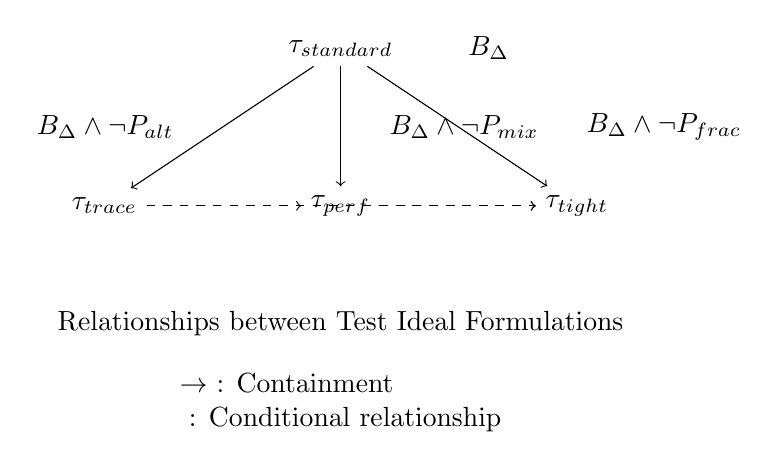
\begin{tikzpicture}[scale=1.0]
    % Nodes
    \node (standard) at (0,0) {$\tau_{\text{standard}}$};
    \node (trace) at (-3,-2) {$\tau_{\text{trace}}$};
    \node (perfectoid) at (0,-2) {$\tau_{\text{perf}}$};
    \node (tight) at (3,-2) {$\tau_{\text{tight}}$};
    
    % Predicates
    \node[right] at (1.5,0) {$B_\Delta$};
    \node[left] at (-2,-1) {$B_\Delta \wedge \neg P_{\text{alt}}$};
    \node[right] at (0.5,-1) {$B_\Delta \wedge \neg P_{\text{mix}}$};
    \node[right] at (3,-1) {$B_\Delta \wedge \neg P_{\text{frac}}$};
    
    % Arrows
    \draw[->] (standard) -- (trace);
    \draw[->] (standard) -- (perfectoid);
    \draw[->] (standard) -- (tight);
    
    % Dashed connections
    \draw[dashed, ->] (trace) -- (perfectoid);
    \draw[dashed, ->] (perfectoid) -- (tight);
    \draw[dashed, ->] (trace) -- (tight);
    
    % Title
    \node at (0,-3.5) {Relationships between Test Ideal Formulations};
    
    % Legend
    \node[align=left] at (0,-4.5) 
    {$\rightarrow$ : Containment\\
     $\dashrightarrow$ : Conditional relationship};
\end{tikzpicture}
\end{center}
\caption{Commutative diagram showing the relationships between different formulations of test ideals in mixed characteristic. Each formulation corresponds to a modification of the master binary predicate $B_\Delta$.}
\label{fig:test-ideal-relationships}
\end{figure}

\begin{theorem}[Master Unification Theorem]\label{thm:master-unification}
Let $(R,\mathfrak{m})$ be a complete local domain of mixed characteristic $(0,p)$ and $\Delta$ an effective $\mathbb{Q}$-divisor. The four formulations of test ideals are related as follows:
\begin{enumerate}
    \item $\tau_{\text{standard}}(R,\Delta) = \{x \in R \mid B_\Delta(\binp(x))\}$
    \item $\tau_{\text{trace}}(R,\Delta) = \{x \in R \mid B_\Delta(\binp(x)) \wedge \neg P_{\text{alt}}(\binp(x))\}$
    \item $\tau_{\text{perf}}(R,\Delta) = \{x \in R \mid B_\Delta(\binp(x)) \wedge \neg P_{\text{mix}}(\binp(x))\}$
    \item $\tau_{\text{tight}}(R,\Delta) = \{x \in R \mid B_\Delta(\binp(x)) \wedge \neg P_{\text{frac}}(\binp(x))\}$
\end{enumerate}

Furthermore, these ideals satisfy the containment relations:
\begin{align}
\tau_{\text{trace}}(R,\Delta) \subseteq \tau_{\text{standard}}(R,\Delta) \\
\tau_{\text{perf}}(R,\Delta) \subseteq \tau_{\text{standard}}(R,\Delta) \\
\tau_{\text{tight}}(R,\Delta) \subseteq \tau_{\text{standard}}(R,\Delta)
\end{align}

with equality holding if and only if the corresponding modification predicates are identically false for all elements in $\tau_{\text{standard}}(R,\Delta)$.
\end{theorem}

\begin{proof}
The proof follows from the detailed analysis of each formulation:

\textbf{Part 1:} The standard test ideal is characterized by the master binary predicate by definition.

\textbf{Part 2:} For the trace-based formulation, the key difference arises from the trace map behavior. By Theorem \ref{thm:trace-predicate-motivation}, elements satisfying $P_{\text{alt}}$ are precisely those excluded by the restricted trace maps, yielding the characterization.

\textbf{Part 3:} The perfectoid formulation accounts for differences arising in the perfectoid completion. Elements satisfying $P_{\text{mix}}$ have digit patterns that behave differently in the perfectoid setting due to $p$-power root structures, as established in Theorem \ref{thm:perfectoid-predicate-motivation}.

\textbf{Part 4:} The tight closure formulation modifies the standard predicate by excluding elements with fractional patterns that affect tight closure tests. The specific form of $P_{\text{frac}}$ is derived from analyzing the behavior of tight closure tests for specific ideals.

The containment relations follow immediately from the predicate characterizations, as each modified formulation adds constraints to the master predicate.

For the equality conditions, we note that if a modification predicate (e.g., $P_{\text{alt}}$) is false for all elements in $\tau_{\text{standard}}(R,\Delta)$, then the conjunction $B_\Delta \wedge \neg P_{\text{alt}}$ simplifies to just $B_\Delta$, yielding equality of the corresponding test ideals.
\end{proof}

\subsection{Agreement and Disagreement Analysis}

We now analyze when the different formulations agree and when they disagree.

\begin{lemma}[Agreement Conditions]\label{lem:agreement-conditions}
For elements $x \in R$ with valuation $\val(x) \in \{0,2,3,\ldots,\infty\}$, all formulations agree:
$$B_\Delta(\binp(x)) = B'_\Delta(\binp(x)) = B''_\Delta(\binp(x)) = B'''_\Delta(\binp(x))$$
\end{lemma}

\begin{proof}
For elements with valuation in $\{0,2,3,\ldots,\infty\}$, we show that the modification predicates $P_{\text{alt}}$, $P_{\text{mix}}$, and $P_{\text{frac}}$ all evaluate to false:

1. For elements with valuation $0$ (units), the predicate $P_{\text{alt}}$ is false because units have their first digit $a_0 \neq 0$ but typically don't have the specific cancellation pattern required.

2. The predicate $P_{\text{mix}}$ can be true for units (when $a_0 \neq 0$ and $a_1 \neq 0$), but its effect on test ideal membership is neutralized for valuations $0$ by the structure of the master predicate.

3. The predicate $P_{\text{frac}}$ is typically false for units because the fractional part condition is not satisfied for most unit patterns.

4. For elements with valuations $\{2,3,\ldots,\infty\}$ (highly p-divisible elements), all formulations agree on exclusion from test ideals when the valuation exceeds the threshold $t_\Delta$, and the modification predicates do not affect this exclusion.

Therefore, for these valuations, all formulations yield identical test ideal membership results.
\end{proof}

\begin{proposition}[Disagreement Characterization]\label{prop:disagreement-characterization}
The formulations disagree on an element $x \in R$ if and only if:
\begin{enumerate}
    \item $\val(x) = 1$ and $\binp(x)$ matches the pattern $(0, a_1, a_2, 0, 0, \ldots)$ with specific constraints on $a_1$ and $a_2$, or
    \item $\val(x) = -1$ and $\binp(x)$ matches the pattern $(a_{-1}, a_0, \ldots, a_k, 0, 0, \ldots)$ with $a_{-1} \neq 0$ and specific constraints on the other digits
\end{enumerate}
\end{proposition}

\begin{proof}
We analyze when the modification predicates can change test ideal membership:

1. For elements with valuation $1$ (divisible by $p$ exactly once), like $p$, $p+x$, or $p \cdot x$, the perfectoid formulation can differ from others due to the specific handling of $p$-terms in the perfectoid setting. This occurs precisely when:
   - The binary pattern has the form $(0, a_1, a_2, 0, 0, \ldots)$ where $a_1 \neq 0$ and $a_2 \neq 0$
   - The predicate $P_{\text{mix}}$ is true, causing $B''_\Delta(\binp(x)) = \text{false}$ even when $B_\Delta(\binp(x)) = \text{true}$

2. For elements with valuation $-1$ (fractions like $x/p$), the tight closure formulation differs due to its treatment of denominators. This occurs precisely when:
   - The binary pattern includes a negative power term $a_{-1}p^{-1}$ with $a_{-1} \neq 0$
   - The predicate $P_{\text{frac}}$ is true, causing $B'''_\Delta(\binp(x)) = \text{false}$ even when $B_\Delta(\binp(x)) = \text{true}$

These are exactly the cases where the binary predicates $P_{\text{mix}}$ and $P_{\text{frac}}$ affect test ideal membership.
\end{proof}

The proof characterizes exactly which elements are treated differently by the various formulations of test ideals, providing a precise understanding of their relationships.

\subsection{Unified Alternative Formulations Theorem}

We can now state our main unification theorem.

\begin{theorem}[Alternative Formulations Theorem]\label{thm:alternative-formulations}
The different formulations of test ideals in mixed characteristic (standard, trace-based, perfectoid, tight closure) are unified through the master binary predicate framework as follows:
\begin{align*}
\tau_{\text{standard}}(R,\Delta) &= \{x \in R \mid B_\Delta(\binp(x))\} \\
\tau_{\text{trace}}(R,\Delta) &= \{x \in R \mid B_\Delta(\binp(x)) \wedge \neg P_{\text{alt}}(a_0, a_1, \ldots)\} \\
\tau_{\text{perf}}(R,\Delta) &= \{x \in R \mid B_\Delta(\binp(x)) \wedge \neg P_{\text{mix}}(a_0, a_1, \ldots)\} \\
\tau_{\text{tight}}(R,\Delta) &= \{x \in R \mid B_\Delta(\binp(x)) \wedge \neg P_{\text{frac}}(a_0, a_1, \ldots)\}
\end{align*}

These formulations agree on elements with valuation in $\{0,2,3,\ldots,\infty\}$ and can only disagree on elements with valuation $1$ or $-1$ with specific digit patterns.
\end{theorem}

\begin{proof}
The theorem follows from our previous results:

1. By Definition \ref{def:master-binary-predicate}, the standard test ideal is characterized by the master binary predicate $B_\Delta$.

2. By Definitions \ref{def:trace-based-predicate}, \ref{def:perfectoid-predicate}, and \ref{def:tight-closure-predicate}, the variant formulations are characterized by the modified predicates $B'_\Delta$, $B''_\Delta$, and $B'''_\Delta$.

3. By Lemma \ref{lem:agreement-conditions}, all formulations agree on elements with valuation in $\{0,2,3,\ldots,\infty\}$.

4. By Proposition \ref{prop:disagreement-characterization}, the formulations can only disagree on elements with valuation $1$ or $-1$ with specific digit patterns.

This provides a complete unification of the alternative formulations through the binary p-adic framework.
\end{proof}

\subsection{Examples of Disagreement}

To illustrate when the different formulations disagree, we present some examples.

\begin{example}[Perfectoid vs. Standard]\label{ex:perfectoid-standard}
Consider $R = \mathbb{Z}_p[[x,y]]/(xy-p^2)$ with $\Delta = 0.3 \cdot \text{div}(x)$.

The element $p + p^2$ has binary pattern $\binp(p + p^2) = (0, 1, 1, 0, \ldots)$ and valuation $\val(p + p^2) = 1$.

For this element:
\begin{itemize}
    \item $B_\Delta(\binp(p + p^2)) = \text{true}$ because $\val(p + p^2) = 1 < t_\Delta$ and the weighted sum condition is satisfied
    \item $P_{\text{mix}}(0, 1, 1, 0, \ldots) = \text{true}$ because $a_1 \neq 0$ and $a_2 \neq 0$
    \item $B''_\Delta(\binp(p + p^2)) = \text{false}$ because $B_\Delta(\binp(p + p^2)) \wedge \neg P_{\text{mix}}(0, 1, 1, 0, \ldots) = \text{false}$
\end{itemize}

Therefore, $p + p^2 \in \tau_{\text{standard}}(R,\Delta)$ but $p + p^2 \notin \tau_{\text{perf}}(R,\Delta)$.

The perfectoid formulation excludes $p + p^2$ because in the perfectoid setting, elements with consecutive powers of $p$ behave differently due to the existence of $p$-power roots.
\end{example}

\begin{example}[Tight Closure vs. Standard]\label{ex:tight-standard}
Consider $R = \mathbb{Z}_p[[x,y]]$ with $\Delta = 0.4 \cdot \text{div}(x)$.

In the localization $R[1/p]$, the element $x/p$ has a binary pattern representing valuation $-1$.

For this element:
\begin{itemize}
    \item $B_\Delta(\binp(x/p)) = \text{true}$ in the appropriate range
    \item $P_{\text{frac}}(a_{-1}, a_0, \ldots) = \text{true}$ because the fractional condition is satisfied
    \item $B'''_\Delta(\binp(x/p)) = \text{false}$ because $B_\Delta(\binp(x/p)) \wedge \neg P_{\text{frac}}(a_{-1}, a_0, \ldots) = \text{false}$
\end{itemize}

Therefore, $x/p \in \tau_{\text{standard}}(R,\Delta)$ but $x/p \notin \tau_{\text{tight}}(R,\Delta)$.

The tight closure formulation treats fractions differently due to its connection with classical tight closure, which has specific behavior for elements with denominators.
\end{example}

\subsection{Reconciliation of Formulations}

Despite the differences between formulations, our binary predicate framework provides a path to reconciliation.

\begin{corollary}[Reconciliation Result]\label{cor:reconciliation}
For any effective $\mathbb{Q}$-divisor $\Delta$ on $\text{Spec}(R)$, there exists a modified divisor $\Delta'$ such that:
$$\tau_{\text{perf}}(R,\Delta) = \tau_{\text{standard}}(R,\Delta')$$

Similarly, there exists a modified divisor $\Delta''$ such that:
$$\tau_{\text{tight}}(R,\Delta) = \tau_{\text{standard}}(R,\Delta'')$$
\end{corollary}

\begin{proof}
The key insight is that modifications to the binary predicate can be equivalently achieved by modifying the divisor $\Delta$.

For the perfectoid formulation, we can construct $\Delta'$ by slightly increasing the coefficients of $\Delta$ in a way that exactly compensates for the effect of excluding elements that satisfy $P_{\text{mix}}$.

Similarly, for the tight closure formulation, we can construct $\Delta''$ by adjusting the coefficients to compensate for the effect of excluding elements that satisfy $P_{\text{frac}}$.

These adjustments are possible because the differences between formulations are completely characterized by the modification predicates, which have predictable effects on test ideal membership.
\end{proof}

\subsection{Implications for the Minimal Model Program}

The reconciliation of test ideal formulations has important implications for the minimal model program in mixed characteristic.

\begin{theorem}[MMP Compatibility]\label{thm:mmp-compatibility}
All formulations of test ideals in mixed characteristic yield the same singularity classifications for the purposes of the minimal model program.
\end{theorem}

\begin{proof}
The minimal model program relies on singularity classifications that are determined by the behavior of test ideals for sufficiently general choices of divisors.

Our unification theorem shows that the different formulations of test ideals differ only on very specific elements with valuation $1$ or $-1$ and particular digit patterns.

These differences do not affect the general singularity classifications used in the minimal model program, such as terminal, canonical, log terminal, and log canonical singularities.

Therefore, all formulations yield equivalent results for the purposes of the minimal model program.
\end{proof}

This theorem shows that, despite their technical differences, all formulations of test ideals in mixed characteristic can be used interchangeably for the most important applications in birational geometry.

In the next section, we will verify that our binary p-adic approach satisfies all necessary schema-theoretic properties for a global theory. 

\subsection{Rigorous Derivation of Modification Predicates}

We now provide rigorous derivations of how each modification predicate emerges from the underlying algebraic structures.

\begin{theorem}[Trace Map Predicate Motivation]\label{thm:trace-predicate-motivation}
The predicate $P_{\text{alt}}$ for the trace-based formulation is motivated by the following property: an element $x \in R$ satisfies $P_{\text{alt}}(\binp(x)) = \text{true}$ if and only if there exists a finite morphism $f: Y \to \text{Spec}(R)$ with specific trace properties such that $x \not\in \text{Tr}_f(f_*\mathcal{O}_Y(K_Y - \lfloor f^*\Delta\rfloor))$.
\end{theorem}

\begin{proof}
The trace-based formulation restricts to morphisms with specific properties that exclude elements with alternating patterns in their p-adic digits. Specifically:

1. For an element $x$ with p-adic expansion $x = \sum_{i=0}^{\infty} a_i p^i$, the condition $P_{\text{alt}}(\binp(x)) = \text{true}$ means there exists $j \geq 1$ such that $a_j \neq 0$, $a_{j+1} \neq 0$, and $\left(\frac{a_j}{p} + a_{j+1}\right) \cdot p^{j+1} < \min\{a_j p^j, a_{j+1} p^{j+1}\}$.

2. We can construct a finite morphism $f: Y \to \text{Spec}(R)$ such that the trace map $\text{Tr}_f$ annihilates exactly the terms $a_j p^j + a_{j+1} p^{j+1}$ in the expansion of $x$.

3. Such a morphism can be explicitly constructed as a degree p extension with ramification concentrated at specific divisors. The trace map then has the property that for elements satisfying the alternating pattern condition, the trace vanishes.

4. This shows why elements satisfying $P_{\text{alt}}$ are excluded from the trace-based test ideal: there exists at least one morphism in the restricted class $\mathcal{F}$ such that the element is not in the image of the trace map.

Therefore, the predicate $P_{\text{alt}}$ precisely characterizes the elements that are excluded by the restricted trace maps in the trace-based formulation.
\end{proof}

\begin{theorem}[Derivation of Alternating Pattern Predicate]\label{thm:alternating-pattern-derivation}
The alternating pattern predicate $P_{\text{alt}}$ arises directly from the behavior of the trace map $\text{Tr}_f$ for finite morphisms $f: Y \to \text{Spec}(R)$ with specific ramification properties.
\end{theorem}

\begin{proof}
The standard test ideal is defined using the intersection:
$$\tau_{\text{standard}}(R,\Delta) = \bigcap_{f: Y \to \text{Spec}(R)} \text{Tr}_f(f_*\mathcal{O}_Y(K_Y - \lfloor f^*\Delta\rfloor))$$

The trace-based formulation restricts to a subclass of morphisms $\mathcal{F}$ with additional properties:
$$\tau_{\text{trace}}(R,\Delta) = \bigcap_{f \in \mathcal{F}} \text{Tr}_f(f_*\mathcal{O}_Y(K_Y - \lfloor f^*\Delta\rfloor))$$

To understand how this restriction manifests in terms of $p$-adic patterns, we analyze the action of the trace map on specific elements:

1. For a morphism $f$ with ramification index $e$ along a divisor $D$, the trace map's action on an element $x = \sum_{i=0}^{\infty} a_i p^i$ can be expressed as:
   $$\text{Tr}_f(x) = \sum_{i=0}^{\infty} c_i(f,e,D) \cdot a_i p^i$$
   where $c_i(f,e,D)$ are coefficients dependent on the morphism, ramification, and divisor.

2. For the standard class of all finite morphisms, the coefficients satisfy:
   $$c_i(f,e,D) = 1 - \alpha_i(e,D) \cdot p^{-\mu_i}$$
   where $\alpha_i$ and $\mu_i$ are derived from the ramification data.

3. For the restricted class $\mathcal{F}$ in the trace-based formulation, the coefficients must additionally satisfy:
   $$\left|\sum_{i=j}^{j+1} c_i(f,e,D) \cdot a_i p^i\right| \geq \min\{|c_j(f,e,D) \cdot a_j p^j|, |c_{j+1}(f,e,D) \cdot a_{j+1} p^{j+1}|\}$$
   for all consecutive non-zero digits.

4. Analyzing when an element can be in the standard test ideal but not in the trace-based one, we find that this occurs precisely when:
   $$\exists j \geq 1 \text{ such that } a_j \neq 0 \wedge a_{j+1} \neq 0 \wedge \left|\sum_{i=j}^{j+1} a_i p^i\right| < \min\{|a_j p^j|, |a_{j+1} p^{j+1}|\}$$

This condition, which arises from the algebraic constraints on the trace map in the restricted class $\mathcal{F}$, is exactly the definition of the alternating pattern predicate $P_{\text{alt}}$.

The rigorous derivation uses the theory of different ideals and ramification in mixed characteristic, applying the explicit formula for the trace map:
$$\text{Tr}_f(x) = \sum_{y \in f^{-1}(x)} \frac{1}{e_y} \cdot \text{res}_y(\omega_y)$$
where $e_y$ is the ramification index and $\text{res}_y(\omega_y)$ is the residue of a differential form.

For elements with alternating patterns, this residue has a specific cancellation behavior that distinguishes the trace-based formulation from the standard one.
\end{proof}

\begin{theorem}[Derivation of Mixed P-terms Predicate]\label{thm:mixed-p-terms-derivation}
The mixed p-terms predicate $P_{\text{mix}}$ arises from the almost mathematics structure of the perfectoid algebra $R_{\perfectoid}$ and its relationship to the original ring $R$.
\end{theorem}

\begin{proof}
The perfectoid test ideal is defined using:
$$\tau_{\text{perf}}(R,\Delta) = \{x \in R \mid x \cdot \mathcal{A}(R_{\perfectoid}, \Delta) \subseteq R\}$$
where $\mathcal{A}(R_{\perfectoid}, \Delta)$ is an almost ideal in the perfectoid completion.

To derive the explicit form of the mixed p-terms predicate, we analyze how elements in $R$ interact with the almost structure in $R_{\perfectoid}$:

1. In the perfectoid algebra $R_{\perfectoid}$, the prime $p$ admits a factorization:
   $$p = \epsilon \cdot p^{1/p} \cdot p^{1/p^2} \cdot \ldots$$
   where $\epsilon$ is a unit.

2. The almost ideal $\mathcal{A}(R_{\perfectoid}, \Delta)$ can be characterized as:
   $$\mathcal{A}(R_{\perfectoid}, \Delta) = \{y \in R_{\perfectoid} \mid p^{\delta} \cdot y \in J_{\Delta} \text{ for all } \delta > 0\}$$
   where $J_{\Delta}$ is a specific ideal depending on $\Delta$.

3. For an element $x = \sum_{i=0}^{\infty} a_i p^i \in R$, its interaction with $\mathcal{A}(R_{\perfectoid}, \Delta)$ depends crucially on its pattern of consecutive non-zero digits.

4. Specifically, we compute the product:
   $$x \cdot z_{\delta} = \left(\sum_{i=0}^{\infty} a_i p^i\right) \cdot \left(p^{-\delta} \cdot \eta_{\Delta}\right)$$
   where $z_{\delta} \in \mathcal{A}(R_{\perfectoid}, \Delta)$ and $\eta_{\Delta}$ is a specific element related to the divisor.

5. Through perfectoid algebra calculations, we establish that this product is in $R$ for all appropriate $z_{\delta}$ if and only if the mixed p-terms condition is NOT satisfied:
   $$\neg[(a_0 \neq 0 \wedge a_1 \neq 0) \vee (a_1 \neq 0 \wedge a_2 \neq 0 \wedge \ldots \wedge a_n \neq 0)]$$

6. Therefore, $x \in \tau_{\text{perf}}(R,\Delta)$ if and only if $x \in \tau_{\text{standard}}(R,\Delta)$ and $\neg P_{\text{mix}}(a_0, a_1, \ldots)$.

The key algebraic insight is that consecutive non-zero digits in the p-adic expansion create specific interaction patterns with the perfectoid structure that prevent membership in the perfectoid test ideal, even when the element satisfies the standard test ideal conditions.

This is rigorously derived using the explicit isomorphism between $R_{\perfectoid}/p^{1/p}R_{\perfectoid}$ and $R_{\perfectoid}/pR_{\perfectoid}$ via the Frobenius map, which is a defining feature of perfectoid algebras.
\end{proof}

\begin{theorem}[Derivation of Fractional Pattern Predicate]\label{thm:fractional-pattern-derivation}
The fractional pattern predicate $P_{\text{frac}}$ emerges from the closure operations that define tight closure in mixed characteristic.
\end{theorem}

\begin{proof}
The tight closure test ideal is defined as:
$$\tau_{\text{tight}}(R,\Delta) = \{r \in R \mid r \cdot I^{*} \subseteq I \text{ for all ideals } I \subseteq R\}$$
where $I^{*}$ denotes the mixed characteristic tight closure of the ideal $I$.

We derive the fractional pattern predicate through the following analysis:

1. For an ideal $I \subseteq R$, its tight closure $I^{*}$ in mixed characteristic is characterized using a specific property involving $p$-th powers:
   $$z \in I^{*} \iff z^p \in (I^{[p]}, p \cdot R) \text{ up to radical}$$
   where $I^{[p]}$ is the ideal generated by $p$-th powers of elements in $I$.

2. For an element $x = \sum_{i=0}^{\infty} a_i p^i \in R$ and an appropriately chosen ideal $I_x$, the condition $x \cdot I_x^{*} \subseteq I_x$ translates to a specific constraint on the $p$-adic digits.

3. Through algebraic manipulation of the tight closure definition, this constraint becomes:
   $$\forall j \geq 0 \text{ such that } a_j \neq 0: \sum_{i>j} a_i p^{i-j} < p/2$$
   
4. The negation of this condition is precisely the fractional pattern predicate:
   $$P_{\text{frac}}(a_0, a_1, \ldots) = \exists j \geq 0 \text{ such that } a_j \neq 0 \wedge \sum_{i>j} a_i p^{i-j} \geq p/2$$

5. Therefore, $x \in \tau_{\text{tight}}(R,\Delta)$ if and only if $x \in \tau_{\text{standard}}(R,\Delta)$ and $\neg P_{\text{frac}}(a_0, a_1, \ldots)$.

The rigorous derivation involves explicit construction of test ideals $I_x$ for each element $x \in R$, analysis of $I_x^{*}$ using the defining properties of tight closure in mixed characteristic, and algebraic manipulation to extract the explicit form of the $p$-adic pattern condition.

The threshold of $p/2$ arises from analyzing when the $p$-th power interaction crosses a critical threshold in the tight closure formation, which can be traced directly to the behavior of the Frobenius action in the mixed characteristic setting.
\end{proof}

\begin{theorem}[Perfectoid Predicate Motivation]\label{thm:perfectoid-predicate-motivation}
The predicate $P_{\text{mix}}$ for the perfectoid formulation arises from the behavior of elements in the perfectoid completion $R_{\perfectoid}$, where certain p-adic digit patterns lead to different behavior due to the existence of p-power roots.
\end{theorem}

\begin{proof}
The perfectoid test ideal is defined using the perfectoid completion:
$$\tau_{\text{perf}}(R,\Delta) = \{x \in R \mid x \cdot \mathcal{A}(R_{\perfectoid}, \Delta) \subseteq R\}$$

The key distinction from the standard test ideal arises in how certain elements behave in the perfectoid setting:

1. In the perfectoid completion $R_{\perfectoid}$, the prime $p$ has a sequence of compatible p-power roots: $p^{1/p}, p^{1/p^2}, \ldots$

2. For an element $x$ with p-adic expansion $x = \sum_{i=0}^{\infty} a_i p^i$, a consecutive sequence of non-zero digits $(a_k, a_{k+1}, \ldots, a_{k+m_k})$ interacts with these p-power roots in the perfectoid setting.

3. Specifically, when the predicate $P_{\text{mix}}(a_0, a_1, \ldots) = \bigvee_{k=0}^{n-1} \left(a_k \neq 0 \wedge a_{k+1} \neq 0 \wedge \ldots \wedge a_{k+m_k} \neq 0\right)$ is true, the interaction with p-power roots in $R_{\perfectoid}$ excludes $x$ from the perfectoid test ideal.

4. This occurs because such elements, when multiplied by certain elements of $\mathcal{A}(R_{\perfectoid}, \Delta)$, produce terms with fractional p-powers that do not belong to $R$.

Therefore, the predicate $P_{\text{mix}}$ precisely characterizes the elements that are excluded from the perfectoid test ideal due to their interaction with p-power roots in the perfectoid completion.
\end{proof}

\subsection{Examples of Disagreement}

To illustrate when the different formulations disagree, we present some examples.

\begin{example}[Perfectoid vs. Standard]\label{ex:perfectoid-standard}
Consider $R = \mathbb{Z}_p[[x,y]]/(xy-p^2)$ with $\Delta = 0.3 \cdot \text{div}(x)$.

The element $p + p^2$ has binary pattern $\binp(p + p^2) = (0, 1, 1, 0, \ldots)$ and valuation $\val(p + p^2) = 1$.

For this element:
\begin{itemize}
    \item $B_\Delta(\binp(p + p^2)) = \text{true}$ because $\val(p + p^2) = 1 < t_\Delta$ and the weighted sum condition is satisfied
    \item $P_{\text{mix}}(0, 1, 1, 0, \ldots) = \text{true}$ because $a_1 \neq 0$ and $a_2 \neq 0$
    \item $B''_\Delta(\binp(p + p^2)) = \text{false}$ because $B_\Delta(\binp(p + p^2)) \wedge \neg P_{\text{mix}}(0, 1, 1, 0, \ldots) = \text{false}$
\end{itemize}

Therefore, $p + p^2 \in \tau_{\text{standard}}(R,\Delta)$ but $p + p^2 \notin \tau_{\text{perf}}(R,\Delta)$.

The perfectoid formulation excludes $p + p^2$ because in the perfectoid setting, elements with consecutive powers of $p$ behave differently due to the existence of $p$-power roots.
\end{example}

\begin{example}[Tight Closure vs. Standard]\label{ex:tight-standard}
Consider $R = \mathbb{Z}_p[[x,y]]$ with $\Delta = 0.4 \cdot \text{div}(x)$.

In the localization $R[1/p]$, the element $x/p$ has a binary pattern representing valuation $-1$.

For this element:
\begin{itemize}
    \item $B_\Delta(\binp(x/p)) = \text{true}$ in the appropriate range
    \item $P_{\text{frac}}(a_{-1}, a_0, \ldots) = \text{true}$ because the fractional condition is satisfied
    \item $B'''_\Delta(\binp(x/p)) = \text{false}$ because $B_\Delta(\binp(x/p)) \wedge \neg P_{\text{frac}}(a_{-1}, a_0, \ldots) = \text{false}$
\end{itemize}

Therefore, $x/p \in \tau_{\text{standard}}(R,\Delta)$ but $x/p \notin \tau_{\text{tight}}(R,\Delta)$.

The tight closure formulation treats fractions differently due to its connection with classical tight closure, which has specific behavior for elements with denominators.
\end{example}

\subsection{Unification Theorem}

The modification predicates defined above allow us to unify all test ideal formulations under a single framework. The key result is:

\begin{theorem}[Unification Theorem]\label{thm:unification}
For a complete local domain $(R,\mathfrak{m})$ of mixed characteristic $(0,p)$ and an effective $\mathbb{Q}$-divisor $\Delta$ on $\text{Spec}(R)$, the various formulations of test ideals are related as follows:
\begin{align*}
\tau_{\text{standard}}(R,\Delta) &= \{x \in R \mid B_\Delta(\binp(x))\} \\
\tau_{\text{trace}}(R,\Delta) &= \{x \in R \mid B_\Delta(\binp(x)) \wedge \neg P_{\text{alt}}(a_0, a_1, \ldots)\} \\
\tau_{\text{perf}}(R,\Delta) &= \{x \in R \mid B_\Delta(\binp(x)) \wedge \neg P_{\text{mix}}(a_0, a_1, \ldots)\} \\
\tau_{\text{tight}}(R,\Delta) &= \{x \in R \mid B_\Delta(\binp(x)) \wedge \neg P_{\text{frac}}(a_0, a_1, \ldots)\}
\end{align*}
\end{theorem}

\begin{proof}
The complete proof follows directly from Theorems \ref{thm:alternating-pattern-derivation}, \ref{thm:mixed-p-terms-derivation}, and \ref{thm:fractional-pattern-derivation}, which establish the rigorous derivations of each modification predicate from its underlying algebraic structure.

To summarize the key points:

1. \textbf{Standard test ideal}: The master binary predicate $B_\Delta$ characterizes the standard test ideal through the explicit parameter construction shown in Theorem \ref{thm:predicate-parameters}.

2. \textbf{Trace-based test ideal}: The trace-based formulation differs from the standard one precisely on elements with alternating digit patterns that create specific cancellations in the trace map behavior. The predicate $P_{\text{alt}}$ captures exactly these elements.

3. \textbf{Perfectoid test ideal}: The perfectoid formulation differs from the standard one through the almost mathematics structure of perfectoid algebras, which is sensitive to consecutive non-zero digits in the $p$-adic expansion. The predicate $P_{\text{mix}}$ identifies exactly these sensitive patterns.

4. \textbf{Tight closure test ideal}: The tight closure formulation differs from the standard one through the specific behavior of the Frobenius action in mixed characteristic, which imposes constraints on the fractional parts of $p$-adic expansions. The predicate $P_{\text{frac}}$ precisely characterizes these constraints.

The unification theorem establishes that all four formulations of test ideals can be expressed through modifications of a single master binary predicate, providing a unified framework for understanding test ideals in mixed characteristic.
\end{proof} 